\subsection{评价区间估计量的方法}\label{sec:9.3}
我们已经见到许多导出置信集的方法，而且对于同一问题，实际上可以导出不同的置信集. 此时当然希望选择最好的一个. 因此，现在考察评价集合估计量的一些方法和准则.

集合估计中，有两个量相互竞争：大小和覆盖概率. 自然希望集合大小较小、覆盖概率较大，但这样的集合通常难以构造.（显然，增大集合就能获得较大的覆盖概率. 区间$(-\infty,\infty)$的覆盖概率为$1$！）在根据大小和覆盖概率优化集合之前，必须决定如何度量这些量.

除特殊情形外，置信集的覆盖概率是参数的函数，因此要考虑的不是一个值，而是无穷多个值. 不过，大多数时候，我们将通过置信系数，即覆盖概率的下确界，来度量覆盖概率的表现.\index{SI0127@置信系数}\semanticindexanchor{127:387} 这是概括覆盖概率信息的一种方式，但并非唯一方式.（例如，也可以计算平均覆盖概率.）

说到置信集的大小，若集合为区间，通常指其长度.\index{SI0188@大小}\semanticindexanchor{188:387} 若集合不是区间，或者处理的是多维集合，那么长度通常变为体积.（也有一些情形，采用长度之外的大小度量更自然，特别是在考虑等变性时. \hyperref[bib:source276]{Schervish 1995}，第6章，以及\hyperref[bib:source18]{Berger 1985}，第6章，讨论了这个主题.）
\subsubsection{大小与覆盖概率}\label{sec:9.3.1}
现在考虑一个看似简单的约束极小化问题：对于给定的覆盖概率，寻找长度最短的置信区间. 先看一个例子.
\begin{example}[长度的优化]\label{ex:9.3.1}
设$X_1,\ldots,X_n$独立同分布于$\mathrm n(\mu,\sigma^2)$，其中$\sigma$已知. 利用\autoref{sec:9.2.2}的方法和
$$Z=\frac{\bar X-\mu}{\sigma/\sqrt n}$$
是服从标准正态分布的枢轴量这一事实，任意满足
$$P(a\le Z\le b)=1-\alpha$$
的$a,b$
\sourcepageanchor{388}
均给出$1-\alpha$置信区间
$$\left\{\mu:\bar x-b\frac\sigma{\sqrt n}\le\mu\le\bar x-a\frac\sigma{\sqrt n}\right\}.$$
哪一对$a,b$最好？更正式地问，怎样选择$a,b$，可以在保持$1-\alpha$覆盖率的同时使置信区间长度最小？注意，置信区间的长度为$(b-a)\sigma/\sqrt n$，但由于每个区间长度都含因子$\sigma/\sqrt n$，可以忽略这一因子，而根据$b-a$的值比较长度. 因而，希望找到一对数$a,b$，使$P(a\le Z\le b)=1-\alpha$，并使$b-a$最小.

在\autoref{ex:9.2.1}中，我们取$a=-z_{\alpha/2},b=z_{\alpha/2}$，但没有提及最优性. 若取$1-\alpha=.90$，则下列任一对数都给出$90\%$区间. \autoref{tab:9.3.3}中的数值研究提示，选择$a=-1.65,b=1.65$给出最好的区间，事实也确实如此. 在这种情形下，平分概率$\alpha$是最优策略.
\par
\begin{table}[htbp]\centering
\setcounter{table}{2}
\caption{三个$90\%$正态置信区间}\label{tab:9.3.3}
\begin{tabular}{rrccr}\toprule
$a$&$b$&\multicolumn{2}{c}{概率}&$b-a$\\\midrule
$-1.34$&$2.33$&$P(Z<a)=.09$&$P(Z>b)=.01$&$3.67$\\
$-1.44$&$1.96$&$P(Z<a)=.075$&$P(Z>b)=.025$&$3.40$\\
$-1.65$&$1.65$&$P(Z<a)=.05$&$P(Z>b)=.05$&$3.30$\\\bottomrule
\end{tabular}
\end{table}
\par
\end{example}
平分$\alpha$的策略在上面的情形中最优，但并不总是最优. 上述情形中，平分$\alpha$之所以最优，是因为pdf在$-z_{\alpha/2}$和$z_{\alpha/2}$处高度相同. 下面证明一个说明此事实的定理；它具有一定的一般性，只需要假设pdf单峰. 回顾单峰（unimodal）的定义：若存在$x^*$，使$f(x)$在$x\le x^*$时非递减，在$x\ge x^*$时非递增，则称pdf $f(x)$单峰.（这是相当弱的要求.）
\begin{theorem}\label{thm:9.3.2}\index{SI0132@最优}\index{SI0135@单峰}
设$f(x)$是单峰pdf. 若区间$[a,b]$满足
\begin{enumerate}[label=\roman*.]
\item\label{item:9.3.2.i}$\int_a^b f(x)\,dx=1-\alpha$，
\item\label{item:9.3.2.ii}$f(a)=f(b)>0$，且
\item\label{item:9.3.2.iii}$a\le x^*\le b$，其中$x^*$为$f(x)$的一个众数，
\end{enumerate}
则$[a,b]$是所有满足\hyperref[item:9.3.2.i]{(a)}的区间中最短的.
\end{theorem}
\begin{proof}
设$[a',b']$是任意满足$b'-a'<b-a$的区间. 将证明这蕴含$\int_{a'}^{b'}f(x)\,dx<1-\alpha$. 只证明$a'\le a$的情形，$a<a'$时证明类似. 还需分两种情形：$b'\le a$和$b'>a$.

若$b'\le a$，则$a'\le b'\le a\le x^*$，且
$$\begin{aligned}
\int_{a'}^{b'}f(x)\,dx
&\le f(b')(b'-a')&&\text{（$x\le b'\le x^*\implies f(x)\le f(b')$）}\\
&\le f(a)(b'-a')&&\text{（$b'\le a\le x^*\implies f(b')\le f(a)$）}\\
&<f(a)(b-a)&&\text{（$b'-a'<b-a$且$f(a)>0$）}\\
&\le\int_a^b f(x)\,dx&&\text{（由\hyperref[item:9.3.2.ii]{(ii)}、\hyperref[item:9.3.2.iii]{(iii)}及单峰性，$a\le x\le b$时$f(x)\ge f(a)$）}\\
&=1-\alpha,&&\text{（\hyperref[item:9.3.2.i]{(i)}）}
\end{aligned}$$
第一种情形得证.
\sourcepageanchor{389}
若$b'>a$，则$a'\le a<b'<b$，因为如果$b'\ge b$，则$b'-a'\ge b-a$. 此时可以写为
$$\begin{aligned}
\int_{a'}^{b'}f(x)\,dx&=\int_a^b f(x)\,dx+\left[\int_{a'}^a f(x)\,dx-\int_{b'}^b f(x)\,dx\right]\\
&=(1-\alpha)+\left[\int_{a'}^a f(x)\,dx-\int_{b'}^b f(x)\,dx\right].
\end{aligned}$$
只要证明方括号内的表达式为负，定理即得证. 利用$f$的单峰性、次序$a'\le a<b'<b$及\hyperref[item:9.3.2.ii]{(b)}，得到
$$\int_{a'}^a f(x)\,dx\le f(a)(a-a')\quad\text{且}\quad\int_{b'}^b f(x)\,dx\ge f(b)(b-b').$$
因而
$$\begin{aligned}
\int_{a'}^a f(x)\,dx-\int_{b'}^b f(x)\,dx
&\le f(a)(a-a')-f(b)(b-b')\\
&=f(a)[(a-a')-(b-b')]\qquad(f(a)=f(b))\\
&=f(a)[(b'-a')-(b-a)],
\end{aligned}$$
当$(b'-a')<(b-a)$且$f(a)>0$时为负.
\end{proof}
若愿意对$f$施加更多假设，例如$f$连续，则可以简化\autoref{thm:9.3.2}的证明. 参见\autoref{exercise:9.38}.

回顾\autoref{ex:9.2.3}之后关于似然区域形式的讨论，\index{SI0134@与最高后验密度的关系}\semanticindexanchor{134:389}由\autoref{thm:9.3.2}现在知道这是一种最优构造. \autoref{cor:9.3.10}给出的类似论证将说明，这种构造如何产生最优贝叶斯区域. 此外，我们现在也可以看出，\autoref{ex:9.3.1}中最优的平分$\alpha$方法，对于任何对称单峰pdf都最优（\autoref{exercise:9.39}）. 即使最优性准则与最小长度有所不同，\autoref{thm:9.3.2}也可能适用.
\begin{example}[期望长度的优化]\label{ex:9.3.3}\index{SI0131@正态}\index{SI0150@正态}
对于基于枢轴量$(\bar X-\mu)/(S/\sqrt n)$的正态区间，我们知道，具有形式
$$\bar x-b\frac s{\sqrt n}\le\mu\le\bar x-a\frac s{\sqrt n}$$
的最短$1-\alpha$置信区间取$a=-t_{n-1,\alpha/2},b=t_{n-1,\alpha/2}$. 区间长度是$s$的函数，一般形式为
$$\operatorname{Length}(s)=(b-a)\frac s{\sqrt n}.$$
容易看出，如果考虑\emph{期望长度}准则，希望找到使
$$E_\sigma(\operatorname{Length}(S))=(b-a)\frac{E_\sigma S}{\sqrt n}=(b-a)c(n)\frac\sigma{\sqrt n}$$
最小的$1-\alpha$区间，那么\autoref{thm:9.3.2}仍适用，选择$a=-t_{n-1,\alpha/2},b=t_{n-1,\alpha/2}$再次给出最优区间.（量$c(n)$是只依赖$n$的常数，参见\autoref{exercise:7.50}.）
\end{example}
在某些情形下，特别是在位置问题以外的场合，应用\autoref{thm:9.3.2}必须谨慎. 尤其在尺度情形中，定理可能无法直接应用，但某个变形可能适用.
\sourcepageanchor{390}
\begin{example}[最短枢轴区间]\label{ex:9.3.4}\index{SI0155@伽马}
设$X\sim\operatorname{gamma}(k,\beta)$. 量$Y=X/\beta$是枢轴量，$Y\sim\operatorname{gamma}(k,1)$，因此可以寻找满足
\begin{equation}\label{eq:9.3.1}P(a\le Y\le b)=1-\alpha\end{equation}
的常数$a,b$来获得置信区间. 不过，盲目应用\autoref{thm:9.3.2}并不能得到最短置信区间. 即选择满足\eqref{eq:9.3.1}及$f_Y(a)=f_Y(b)$的$a,b$并非最优. 因为基于\eqref{eq:9.3.1}的$\beta$区间具有形式
$$\left\{\beta:\frac xb\le\beta\le\frac xa\right\},$$
所以区间长度为$(1/a-1/b)x$，即与$(1/a)-(1/b)$成正比，而不是与$b-a$成正比.

虽然\autoref{thm:9.3.2}不能直接应用，但修改论证可以解决这个问题. \autoref{thm:9.3.2}的\hyperref[item:9.3.2.i]{条件(i)}将$b$定义为$a$的函数，记为$b(a)$. 必须解以下约束极小化问题：
$$\begin{aligned}
\text{关于$a$极小化：}\quad&\frac1a-\frac1{b(a)}\\
\text{约束条件：}\quad&\int_a^{b(a)}f_Y(y)\,dy=1-\alpha.
\end{aligned}$$
对第一个式子关于$a$求导，并令导数为零，得到恒等式$db/da=b^2/a^2$. 将其代入第二个式子的导数（该导数必为零），得到$f(b)b^2=f(a)a^2$（\autoref{exercise:9.42}）. 正态分布方差的区间估计中也会出现这样的方程，参见\autoref{ex:9.2.10}和\autoref{exercise:9.52}. 注意，上述方程定义的不是总体意义下最短的区间，而是最短枢轴区间，即基于枢轴量$X/\beta$的最短区间. 涉及Neyman--Pearson引理的推广见\autoref{exercise:9.43}.
\end{example}
\subsubsection{与检验相关的最优性}\label{sec:9.3.2}
由于置信集与假设检验一一对应（\autoref{thm:9.2.2}），检验的最优性与置信集的最优性也存在某种对应关系. 通常，置信集与检验相关的最优性质并不直接涉及集合大小，而是涉及集合覆盖错误值的概率.

覆盖错误值的概率，或称错误覆盖概率（probability of false coverage），间接度量置信集的大小. 直觉上，较小的集合覆盖的值较少，因此覆盖错误值的可能性也较小. 此外，后面还将看到联系大小与错误覆盖概率的方程.

先考虑一般情形，$\boldsymbol X\sim f(\boldsymbol x\mid\theta)$，通过反演接受域$A(\theta)$，构造$\theta$的$1-\alpha$置信集$C(\boldsymbol x)$. $C(\boldsymbol x)$的覆盖概率，即正确覆盖概率，为$\theta$的函数$P_\theta(\theta\in C(\boldsymbol X))$. 错误覆盖概率是$\theta$和$\theta'$的函数，定义为
\begin{equation}\label{eq:9.3.2}\index{SI0858@错误覆盖概率}
\begin{aligned}
P_\theta(\theta'\in C(\boldsymbol X)),\ \theta\ne\theta',&\qquad\text{若 }C(\boldsymbol X)=[L(\boldsymbol X),U(\boldsymbol X)],\\
P_\theta(\theta'\in C(\boldsymbol X)),\ \theta'<\theta,&\qquad\text{若 }C(\boldsymbol X)=[L(\boldsymbol X),\infty),\\
P_\theta(\theta'\in C(\boldsymbol X)),\ \theta'>\theta,&\qquad\text{若 }C(\boldsymbol X)=(-\infty,U(\boldsymbol X)],
\end{aligned}
\end{equation}
即$\theta$是真实参数时覆盖$\theta'$的概率.

对单侧和双侧区间采用不同的错误覆盖概率定义是合理的. 例如，有置信下界时，我们断言$\theta$大于某个值，只有当覆盖了过小的$\theta$值时才会发生错误覆盖. 类似论证导出置信上界与双侧界所用的定义.
\sourcepageanchor{391}
若一个$1-\alpha$置信集在某类$1-\alpha$置信集中使错误覆盖概率最小，则称其为一致最精确置信集（uniformly most accurate，UMA）.\index{SI0189@一致最准确}\semanticindexanchor{189:391} 例如，可以考虑在$[L(\boldsymbol x),\infty)$形式的集合中寻找UMA置信集. UMA置信集可通过反演UMP检验的接受域构造，下面将证明这一点. 遗憾的是，虽然UMA置信集很理想，但它只在相当少见的情形下存在（UMP检验也如此）. 特别地，由于UMP检验通常是单侧的，UMA区间也通常为单侧. 不过，它们构成了优美的理论. 下一个定理说明，$H_0:\theta=\theta_0$对$H_1:\theta>\theta_0$的UMP检验给出UMA置信下界.
\begin{theorem}\label{thm:9.3.5}\index{SI0191@与一致最强检验的关系}\index{SI0518@与一致最准确集的关系}
设$\boldsymbol X\sim f(\boldsymbol x\mid\theta)$，其中$\theta$为实值参数. 对每个$\theta_0\in\Theta$，设$A^*(\theta_0)$是$H_0:\theta=\theta_0$对$H_1:\theta>\theta_0$的水平$\alpha$ UMP检验的接受域. 设$C^*(\boldsymbol x)$为反演这些UMP接受域所得的$1-\alpha$置信集. 则对于任何其他$1-\alpha$置信集$C$，
$$P_\theta(\theta'\in C^*(\boldsymbol X))\le P_\theta(\theta'\in C(\boldsymbol X)),\qquad\text{对所有 }\theta'<\theta.$$
\end{theorem}
\begin{proof}
设$\theta'$为小于$\theta$的任意值. 设$A(\theta')$是反演$C$得到的$H_0:\theta=\theta'$的水平$\alpha$检验的接受域. 因为$A^*(\theta')$是检验$H_0:\theta=\theta'$对$H_1:\theta>\theta'$的UMP接受域，且$\theta>\theta'$，所以
$$\begin{aligned}
P_\theta(\theta'\in C^*(\boldsymbol X))&=P_\theta(\boldsymbol X\in A^*(\theta'))&&\text{（反演置信集）}\\
&\le P_\theta(\boldsymbol X\in A(\theta'))&&\text{（$A^*$为UMP，故对任意$A$成立）}\\
&=P_\theta(\theta'\in C(\boldsymbol X)).&&\text{（反演$A$得到$C$）}
\end{aligned}$$
注意，上述不等号为“$\le$”，因为我们处理的是接受域的概率. 它等于$1-\text{功效}$，所以UMP检验使接受域的概率最小. 因而已证明，当$\theta'<\theta$时，反演UMP检验所得区间使错误覆盖概率最小.
\end{proof}
回顾\autoref{sec:9.2.1}中的讨论. 上述定理的UMA置信集通过反演下列假设的一族检验构造：
$$H_0:\theta=\theta_0\qquad\text{对}\qquad H_1:\theta>\theta_0,$$
其中置信集的形式由备择假设决定. 上述备择假设规定$\theta_0$小于某个特定值，因此产生置信下界；即如果集合是区间，它们就具有$[L(\boldsymbol X),\infty)$的形式.
\begin{example}[UMA置信界]\label{ex:9.3.6}\index{SI0190@正态}
设$X_1,\ldots,X_n$独立同分布于$\mathrm n(\mu,\sigma^2)$，其中$\sigma^2$已知. 区间
$$C(\bar x)=\left\{\mu:\mu\ge\bar x-z_\alpha\frac\sigma{\sqrt n}\right\}$$
是$1-\alpha$ UMA置信下界，因为它可通过反演$H_0:\mu=\mu_0$对$H_1:\mu>\mu_0$的UMP检验得到.

更常见的双侧区间
$$C(\bar x)=\left\{\mu:\bar x-z_{\alpha/2}\frac\sigma{\sqrt n}\le\mu\le\bar x+z_{\alpha/2}\frac\sigma{\sqrt n}\right\}$$
不是UMA，因为它来自$H_0:\mu=\mu_0$对$H_1:\mu\ne\mu_0$检验的双侧接受域反演，而对于这组假设，不存在UMP检验.
\end{example}
\sourcepageanchor{392}
在检验问题中考虑双侧检验时，我们发现无偏性既令人信服又有用. 置信区间问题中也有类似思想. 处理双侧置信区间时，将考虑范围限于无偏置信集是合理的. 记住，无偏检验的备择假设下的功效总大于原假设下的功效. 阅读下面定义时请牢记这一点.
\begin{definition}\label{def:9.3.7}\index{SI0192@无偏}
若一个$1-\alpha$置信集$C(\boldsymbol x)$对所有$\theta\ne\theta'$均满足$P_\theta(\theta'\in C(\boldsymbol X))\le1-\alpha$，则称其无偏（unbiased）.
\end{definition}
因此，对于无偏置信集，错误覆盖概率决不会大于最小正确覆盖概率. 无偏置信集可通过反演无偏检验得到.\index{SI0194@与无偏检验的关系}\semanticindexanchor{194:392}\index{SI0521@与无偏集的关系}\semanticindexanchor{521:392} 即若$A(\theta_0)$是检验$H_0:\theta=\theta_0$对$H_1:\theta\ne\theta_0$的无偏水平$\alpha$接受域，且$C(\boldsymbol x)$是反演这些接受域形成的$1-\alpha$置信集，则$C(\boldsymbol x)$是无偏$1-\alpha$置信集（\autoref{exercise:9.46}）.
\begin{example}[续\autoref{ex:9.3.6}]\label{ex:9.3.8}\index{SI0193@正态}
双侧正态区间
$$C(\bar x)=\left\{\mu:\bar x-z_{\alpha/2}\frac\sigma{\sqrt n}\le\mu\le\bar x+z_{\alpha/2}\frac\sigma{\sqrt n}\right\}$$
是无偏区间. 它可通过反演\autoref{ex:8.3.20}给出的$H_0:\mu=\mu_0$对$H_1:\mu\ne\mu_0$的无偏检验得到. 类似地，基于$t$分布的区间\eqref{eq:9.2.14}也是无偏区间，因为它也可以通过反演无偏检验得到（\autoref{exercise:8.38}）.
\end{example}
使错误覆盖概率最小的集合也称为Neyman最短（Neyman-shortest）集合.\index{SI0721@Neyman最短}\semanticindexanchor{721:392} 这个名称包含长度的意味，\hyperref[bib:source246]{Pratt（1961）}的下述定理为其提供了某种依据.
\begin{theorem}[Pratt]\label{thm:9.3.9}\index{SI0133@与错误覆盖的关系}\index{SI0822@Pratt定理}
设$X$是实值随机变量，$X\sim f(x\mid\theta)$，其中$\theta$是实值参数. 设$C(x)=[L(x),U(x)]$是$\theta$的置信区间. 若$L(x)$和$U(x)$均为$x$的递增函数，则对任意值$\theta^*$，
\begin{equation}\label{eq:9.3.3}
E_{\theta^*}(\operatorname{Length}[C(X)])=\int_{\theta\ne\theta^*}P_{\theta^*}(\theta\in C(X))\,d\theta.
\end{equation}
\end{theorem}
\autoref{thm:9.3.9}表明，$C(x)$的期望长度等于错误覆盖概率之和（积分），其中积分遍及参数的所有错误值.
\begin{proof}
根据期望值的定义，可以写为
$$\begin{aligned}
E_{\theta^*}(\operatorname{Length}[C(X)])
&=\int_{\mathcal X}\operatorname{Length}[C(x)]f(x\mid\theta^*)\,dx\\
&=\int_{\mathcal X}[U(x)-L(x)]f(x\mid\theta^*)\,dx&&\text{（长度的定义）}\\
&=\int_{\mathcal X}\left[\int_{L(x)}^{U(x)}d\theta\right]f(x\mid\theta^*)\,dx&&\text{（用$\theta$作积分变量）}\\
&=\int_\Theta\left[\int_{U^{-1}(\theta)}^{L^{-1}(\theta)}f(x\mid\theta^*)\,dx\right]d\theta&&\text{（交换积分次序，见下文）}\\
&=\int_\Theta[P_{\theta^*}(U^{-1}(\theta)\le X\le L^{-1}(\theta))]\,d\theta&&\text{（定义）}\\
&=\int_\Theta[P_{\theta^*}(\theta\in C(X))]\,d\theta&&\text{（反演接受域）}\\
&=\int_{\theta\ne\theta^*}[P_{\theta^*}(\theta\in C(X))]\,d\theta.&&\text{（一个点不改变积分值）}
\end{aligned}$$
\sourcepageanchor{393}
这串等式建立了所需恒等式，定理得证. 积分次序的交换形式上由Fubini定理保证（\hyperref[bib:source200]{Lehmann和Casella 1998}，第1.2节），但只要所有被积函数有限，就容易看出交换是合理的.\footnote{译注：一般而言，仅要求被积函数处处有限不足以保证交换积分次序；这里的被积函数非负，交换可由Tonelli定理得到（容许积分为无穷）. 原文表述保留.} 置信区间的反演是标准的，其中使用关系
$$\theta\in\{\theta:L(x)\le\theta\le U(x)\}\iff x\in\{x:U^{-1}(\theta)\le x\le L^{-1}(\theta)\},$$
它因$L,U$递增的假设而成立. 注意，修改定理后也可适用于端点递减的区间.
\end{proof}
\autoref{thm:9.3.9}说明，置信区间的长度与错误覆盖概率之间存在形式上的关系. 在双侧情形中，这意味着使错误覆盖概率最小也带来某种长度最优保证. 不过，在单侧情形中，这种类比并不完全成立. 此时，为使错误覆盖概率最小而构造的区间，只关注参数空间一部分中的参数，因而可能没有长度最优性. \hyperref[bib:source213]{Madansky（1962）}给出了一个可被改进的$1-\alpha$ UMA单侧区间例子：可以构造另一个更短的$1-\alpha$区间.（参见\autoref{exercise:9.45}.）此外，\hyperref[bib:source212]{Maatta和Casella（1987）}证明，反演UMP检验所得区间，按其他合理准则衡量时可能并非最优.
\subsubsection{贝叶斯最优性}\label{sec:9.3.3}
获得具有指定覆盖概率的最小置信集这一目标，也可借助贝叶斯准则实现. 若有后验分布$\pi(\theta\mid\boldsymbol x)$，即给定$\boldsymbol X=\boldsymbol x$时$\theta$的后验分布，我们希望找到集合$C(\boldsymbol x)$，使
\begin{enumerate}[label=\roman*.]
\item $\displaystyle\int_{C(\boldsymbol x)}\pi(\theta\mid\boldsymbol x)\,d\boldsymbol x=1-\alpha$；
\item $\operatorname{Size}(C(\boldsymbol x))\le\operatorname{Size}(C'(\boldsymbol x))$，
\end{enumerate}
其中$C'(\boldsymbol x)$为任意满足$\int_{C'(\boldsymbol x)}\pi(\theta\mid\boldsymbol x)\,d\boldsymbol x\ge1-\alpha$的集合.\footnote{译注：原文以上两处后验积分的微分均写作$d\boldsymbol x$；积分区域是参数集合，因此应为$d\theta$. 此处保留原式.}

如果以长度作为大小的度量，则可以应用\autoref{thm:9.3.2}，得到如下结果.
\begin{corollary}\label{cor:9.3.10}\index{SI0471@最高后验密度区域}
若后验密度$\pi(\theta\mid\boldsymbol x)$单峰，则对于给定$\alpha$，$\theta$的最短可信区间为
$$\{\theta:\pi(\theta\mid\boldsymbol x)\ge k\},\qquad\text{其中}\quad\int_{\{\theta:\pi(\theta\mid\boldsymbol x)\ge k\}}\pi(\theta\mid\boldsymbol x)\,d\theta=1-\alpha.$$
\end{corollary}
\autoref{cor:9.3.10}所述的可信集称为最高后验密度区域（highest posterior density region，HPD区域），因为它由后验密度最高的参数值组成. 注意HPD区域与似然区域在形式上的相似性.
\begin{example}[泊松HPD区域]\label{ex:9.3.11}
在\autoref{ex:9.2.16}中，我们导出了泊松参数的$1-\alpha$可信集. 现在构造HPD区域. 由\autoref{cor:9.3.10}，此区域为$\{\lambda:\pi(\lambda\mid\sum x)\ge k\}$，其中$k$选取为使
$$1-\alpha=\int_{\{\lambda:\pi(\lambda\mid\sum x)\ge k\}}\pi(\lambda\mid\textstyle\sum x)\,d\lambda.$$
回顾$\lambda$的后验pdf为$\operatorname{gamma}(a+\sum x,[n+(1/b)]^{-1})$，因此需要找到$\lambda_L,\lambda_U$使\footnote{译注：原文在两个端点密度$\pi(\lambda_L\mid\sum x)$和$\pi(\lambda_U\mid\sum x)$之间漏印关系符号；由HPD区域的等高端点条件，此处应为等号. 原式保留.}
$$\pi(\lambda_L\mid\textstyle\sum x)\pi(\lambda_U\mid\textstyle\sum x)\quad\text{且}\quad\int_{\lambda_L}^{\lambda_U}\pi(\lambda\mid\textstyle\sum x)\,d\lambda=1-\alpha.$$

\sourcepageanchor{394}
若取$a=b=1$（与\autoref{ex:9.2.16}相同），则给定$\sum X=\sum x$时$\lambda$的后验分布可表示为$2(n+1)\lambda\sim\chi^2_{2(\sum x+1)}$；若$n=10$且$\sum x=6$，则$\lambda$的$90\%$ HPD可信集为$[.253,1.005]$.

\autoref{fig:9.3.1}展示了$\lambda$的三个$1-\alpha$区间：\autoref{ex:9.2.16}中的$1-\alpha$等尾贝叶斯可信集、这里导出的HPD区域，以及\autoref{ex:9.2.15}中的经典$1-\alpha$置信集.
\par
\begin{figure}[htbp]\centering
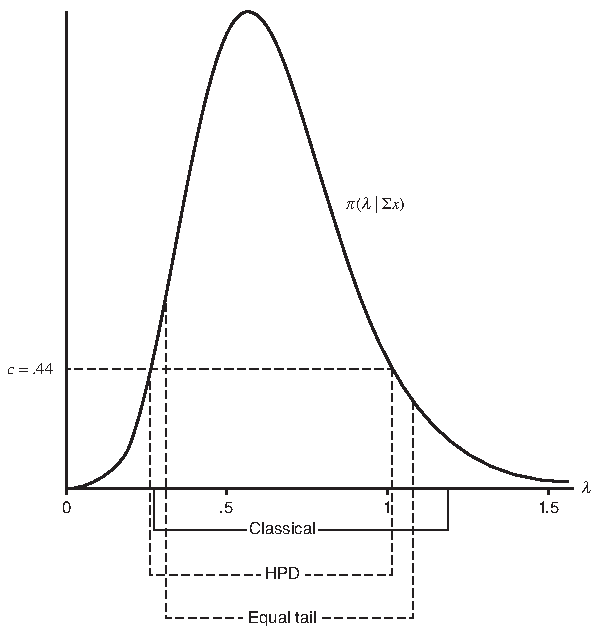
\includegraphics[width=.72\textwidth]{assets/chapter9/fig-9.3.1.pdf}
\caption{\autoref{ex:9.2.16}中的三个区间估计量.}\label{fig:9.3.1}
\end{figure}
\par
\end{example}
HPD区域的形状由后验分布的形状决定. 一般地，HPD区域并不关于某个贝叶斯点估计量对称，而是像似然区域一样相当不对称. 对泊松分布，这显然成立，如上例所示. 尽管不总如此，但通常可预期：尺度参数问题产生不对称HPD区域，位置参数问题产生对称HPD区域.
\begin{example}[正态HPD区域]\label{ex:9.3.12}
\autoref{ex:9.2.18}导出的等尾可信集实际上是HPD区域. 因为$\theta$的后验分布是均值为$\delta^{\mathrm B}$的正态分布，所以对某个$k'$有（\autoref{exercise:9.40}）$\{\theta:\pi(\theta\mid\bar x)\ge k\}=\{\theta:\theta\in\delta^{\mathrm B}\pm k'\}$. 因而HPD区域关于均值$\delta^{\mathrm B}(\bar x)$对称.
\end{example}
\subsubsection{损失函数意义下的最优性}\label{sec:9.3.4}
前两小节研究区间估计量最优性时，先要求它们具有某个最小覆盖概率，然后寻找最短区间. 不过，
\sourcepageanchor{395}
也可以将这些要求合并到一个损失函数中，利用决策论寻找最优估计量. 在区间估计中，行动空间$\mathcal A$由参数空间$\Theta$的子集构成；更正式地说，我们或许应称之为“集合估计”，因为最优规则未必是区间. 然而，出于实际考虑，我们主要研究以区间为集合估计量的情形；幸运的是，许多最优程序最终确实是区间.

用$C$（取自置信区间）表示$\mathcal A$中的元素，行动$C$的含义是作出区间估计“$\theta\in C$\mbox{”.} 决策规则$\delta(\boldsymbol x)$仅仅规定：对每个$\boldsymbol x\in\mathcal X$，若观测到$\boldsymbol X=\boldsymbol x$，将用哪个集合$C\in\mathcal A$估计$\theta$. 因此，仍沿用记号$C(\boldsymbol x)$.

区间估计问题的损失函数通常包括两个量：集合估计是否正确包含真值$\theta$的度量，以及集合估计大小的度量. 大多数时候只考虑作为区间的集合$C$，因而一个自然的大小度量是$\operatorname{Len}(C)=C\text{的长度}$. 为表示正确性度量，通常用
$$I_C(\theta)=\begin{cases}1,&\theta\in C,\\0,&\theta\notin C.\end{cases}$$
即估计正确时$I_C(\theta)=1$，否则为零. 事实上，$I_C(\theta)$就是集合$C$的示性函数. 但应注意，$C$将是由数据$\boldsymbol X$的值决定的随机集合.

损失函数应反映良好估计具有较小$\operatorname{Len}(C)$和较大$I_C(\theta)$这一事实. 一种这样的损失函数是
\begin{equation}\label{eq:9.3.4}\index{SI0146@决策论}\index{SI0657@区间估计}
L(\theta,C)=b\operatorname{Length}(C)-I_C(\theta),
\end{equation}
其中$b$为正常数，反映我们希望赋予两个准则的相对权重；由于这两个量很不相同，这种权衡是必要的. 若更关注估计正确，应取较小的$b$；若更关注区间长度，则应取较大的$b$.

与\eqref{eq:9.3.4}对应的风险函数特别简单：
$$\begin{aligned}
R(\theta,C)&=bE_\theta[\operatorname{Length}(C(\boldsymbol X))]-E_\theta I_{C(\boldsymbol X)}(\theta)\\
&=bE_\theta[\operatorname{Length}(C(\boldsymbol X))]-P_\theta(I_{C(\boldsymbol X)}(\theta)=1)\\
&=bE_\theta[\operatorname{Length}(C(\boldsymbol X))]-P_\theta(\theta\in C(\boldsymbol X)).
\end{aligned}$$
风险有两部分：区间的期望长度和区间估计量的覆盖概率.\index{SI0128@与风险的关系}\semanticindexanchor{128:395}\index{SI0226@与风险的关系}\semanticindexanchor{226:395} 风险反映了与前面各小节相同的愿望：同时希望期望长度小、覆盖概率高. 但现在不再先要求最低覆盖概率、再极小化长度，而是在风险函数中规定这两个量的权衡. 如果能显著缩短长度，较小的覆盖概率也许可以接受.

改变损失\eqref{eq:9.3.4}中$b$的大小，就能改变区间估计量的大小与覆盖概率的相对重要性，这是此前无法做到的. 为展示当前框架的灵活性，考虑某些极限情形. 若$b=0$，则大小不重要，只有覆盖概率重要，因此覆盖概率为$1$的区间估计量$C=(-\infty,\infty)$是最佳决策规则. 类似地，若$b=\infty$，则覆盖概率不重要，因此单点集合最优. 于是，一整系列决策规则都可能成为候选. 下例中，对于某个指定的有限$b$值范围，选择良好规则归结为用风险函数确定置信系数；如果$b$在此范围外，则最优决策规则是点估计量.
\begin{example}[正态区间估计量]\label{ex:9.3.13}\index{SI0148@均值}
设$X\sim\mathrm n(\mu,\sigma^2)$，假设$\sigma^2$已知. $X$通常是样本均值，而$\sigma^2$具有$\tau^2/n$的形式，其中$\tau^2$为已知总体方差，$n$为样本量. 对每个$c\ge0$，定义$\mu$的区间估计量$C(x)=[x-c\sigma,x+c\sigma]$. 将利用\eqref{eq:9.3.4}中的损失比较这些估计量. 区间的
\sourcepageanchor{396}
长度$\operatorname{Len}(C(x))=2c\sigma$不依赖$x$. 因此，风险第一项为$b(2c\sigma)$. 第二项为
$$\begin{aligned}
P_\mu(\mu\in C(X))&=P_\mu(X-c\sigma\le\mu\le X+c\sigma)\\
&=P_\mu\left(-c\le\frac{X-\mu}\sigma\le c\right)\\
&=2P(Z\le c)-1,
\end{aligned}$$
其中$Z\sim\mathrm n(0,1)$. 因而，这一类区间估计量的风险函数为
\begin{equation}\label{eq:9.3.5}
R(\mu,C)=b(2c\sigma)-[2P(Z\le c)-1].
\end{equation}
风险函数不依赖$\mu$，所以是常数；此类中最佳区间估计量对应于使\eqref{eq:9.3.5}最小的$c$值.

若$b\sigma>1/\sqrt{2\pi}$，可证明$R(\mu,C)$在$c=0$时最小. 即损失中长度部分完全压倒了覆盖概率部分，最佳区间估计量是点估计量$C(x)=[x,x]$. 但若$b\sigma\le1/\sqrt{2\pi}$，则风险在$c=\sqrt{-2\log(b\sigma\sqrt{2\pi})}$处最小. 若将$c$写成某个$\alpha$对应的$z_{\alpha/2}$，则使风险最小的区间估计量恰是通常的$1-\alpha$置信区间.（细节见\autoref{exercise:9.53}.）
\end{example}
决策论在区间估计问题中的应用，不像在点估计或假设检验问题中那样广泛.\index{SI0147@困难}\semanticindexanchor{147:396} 一个原因是\eqref{eq:9.3.4}（或\autoref{ex:9.3.13}）中的$b$难以选择. 上例说明，一个看似合理的选择可能产生不符合直觉的结果，表明\eqref{eq:9.3.4}中的损失可能不适当. 有些人在其他问题中使用决策论分析，但仍倾向于仅使用置信系数固定为$1-\alpha$的区间估计量，然后用风险函数评价集合大小等其他品质.

另一个困难在于对$\mathcal A$中允许集合形状的限制. 理想地，应由损失和风险函数判断哪些形状最好. 但总可以向区间估计量加入孤立点，在大小方面不受损失惩罚，却提高覆盖概率. 上例中本可以使用估计量
$$C(x)=[x-c\sigma,x+c\sigma]\cup\{\mu\text{的所有整数值}\}.$$
这些集合的“长度”与此前相同，但现在对$\mu$的所有整数值，覆盖概率都是$1$. 必须采用更精细的大小度量才能避免此类反常现象.（\hyperref[bib:source183]{Joshi 1969}通过定义估计量的等价类处理了这个问题.）
